\documentclass[11pt,a4paper]{article}
\usepackage[utf8]{inputenc}
\usepackage[margin=1in]{geometry}
\usepackage{amsmath,amssymb,amsfonts}
\usepackage{graphicx}
\usepackage{booktabs}
\usepackage{array}
\usepackage{xcolor}
\usepackage{hyperref}
\usepackage{fancyhdr}
\usepackage{caption}
\usepackage{subcaption}
\usepackage{float}
\usepackage{titlesec}
\usepackage{enumitem}

% Color Definitions
\definecolor{primary}{RGB}{20, 50, 90}     % Deep Navy
\definecolor{secondary}{RGB}{40, 100, 150} % Muted Blue
\definecolor{accent}{RGB}{180, 50, 50}     % Deep Red/Burgundy
\definecolor{bglight}{RGB}{245, 247, 250}  % Light Gray-Blue

% Header & Footer Setup
\pagestyle{fancy}
\fancyhf{}
\rhead{\textcolor{secondary}{\small Interim Report: UDCA Nanosuspension}}
\lhead{\textcolor{secondary}{\small IIT Bombay -- Synochem Pharma}}
\rfoot{\thepage}
\lfoot{\textcolor{secondary}{\small Confidential}}
\renewcommand{\headrulewidth}{0.4pt}
\renewcommand{\footrulewidth}{0.4pt}

% Hyperlink styling
\hypersetup{
    colorlinks=true,
    linkcolor=primary,
    citecolor=secondary,
    urlcolor=secondary
}

% Section styling
\titleformat{\section}{\color{primary}\large\bfseries}{\thesection}{1em}{}[\hline]
\titleformat{\subsection}{\color{secondary}\bfseries}{\thesubsection}{1em}{}

\begin{document}

% Title Page / Header Block
\begin{titlepage}
    \centering
    \vspace*{1cm}
    {\Huge \bfseries Interim Technical Report \par}
    \vspace{0.5cm}
    {\Large \color{secondary} Preparation and Characterization of Nanosuspension of Ursodeoxycholic Acid (UDCA) from Micronized Particles \par}
    \vspace{1.5cm}
    
    \textbf{Prepared for:}\\
    \Large Synochem Pharma\\
    \vspace{1cm}
    
    \textbf{Investigators:}\\
    \Large Prof. Rochish M. Thaokar\\
    Sneha Borde\\
    \vspace{0.5cm}
    \small Department of Chemical Engineering\\
    Indian Institute of Technology Bombay (IIT Bombay)\\
    
    \vfill
    
    {\large \today \par}
\end{titlepage}

\newpage

\section{Executive Summary}
Ursodeoxycholic acid (UDCA) is a hydrophobic bile acid drug used in treating liver conditions, including cholelithiasis (gallstones) and primary biliary cholangitis. Due to its exceptionally poor aqueous solubility, its oral bioavailability is severely limited. Particle size reduction down to the nanometer range increases specific surface area, thereby enhancing dissolution rates and biological absorption. 

This interim report summarizes the collaborative research project between IIT Bombay and Synochem Pharma aimed at converting micronized UDCA particles into stable nanometer-scale powders/suspensions. Various bottom-up (anti-solvent precipitation, electrospray, lyophilization) and top-down (high-pressure homogenization, ball milling) processes have been investigated alongside particle characterization techniques (Dynamic Light Scattering [DLS] and Scanning Electron Microscopy [SEM]).

\section{Problem Statement \& Objectives}
\begin{description}[style=multiline,leftmargin=3.5cm]
    \item[Problem Statement:] UDCA exhibits high hydrophobicity, leading to poor aqueous solubility, reduced dissolution kinetics, and sub-optimal bioavailability.
    \item[Project Objective:] To reduce micronized UDCA active pharmaceutical ingredients (API) to the sub-micron/nanometer scale ($<500\text{ nm}$) and formulate a stable, water-dispersible nanosized powder or suspension.
\end{description}

\section{Approaches \& Methodology}
To accomplish particle size reduction and stabilization, both top-down and bottom-up methodologies were evaluated:

\begin{enumerate}
    \item \textbf{Bottom-Up Approaches:}
    \begin{itemize}
        \item \textbf{Anti-Solvent Precipitation:} Dissolution of UDCA in an organic solvent (IPA/Ethanol) at elevated temperatures followed by controlled dropwise addition into an aqueous anti-solvent phase (with/without Hydroxypropyl Methylcellulose [HPMC] stabilizer).
        \item \textbf{Electrospraying:} Atomization of UDCA-solvent solution under a high-voltage DC electric field ($3$--$4\text{ kV}$) to produce ultrafine aerosolized particles collected on an electrode.
        \item \textbf{Lyophilization (Freeze-Drying):} Solubilization of UDCA in alkaline solution ($\text{NaOH}$), acid precipitation ($\text{HCl}$) with HPMC, followed by structured multi-stage freezing ($-80^\circ\text{C}$ to $+10^\circ\text{C}$) and sublimation.
    \end{itemize}
    \item \textbf{Top-Down Approaches:}
    \begin{itemize}
        \item \textbf{High-Pressure Homogenization (HPH):} Mechanical cavitation/shear processing using 50 cycles at 1500 RPM with active cooling.
        \item \textbf{Ball Milling:} Dry and wet media milling (under optimization).
    \end{itemize}
\end{enumerate}

\section{Characterization of Raw UDCA Active Material}
Preliminary analysis of raw UDCA was performed using DLS and SEM. 

\begin{table}[H]
\centering
\caption{DLS Characterization Data for Raw UDCA in Water}
\begin{tabular}{ll}
\toprule
\textbf{Parameter} & \textbf{Value} \\
\midrule
Hydrodynamic Diameter ($D_h$) & $1268.3\text{ nm} - 1602.8\text{ nm}$ \\
Polydispersity Index (PDI) & $29.6\% - 81.4\%$ \\
Diffusion Coefficient & $0.3 - 0.4\ \mu\text{m}^2/\text{s}$ \\
Peak 1 Diameter (51.1\% area) & $995.5\text{ nm}$ \\
Peak 2 Diameter (48.9\% area) & $7517\text{ nm}$ \\
\bottomrule
\end{tabular}
\end{table}

\paragraph{Analytical Note / Caution:} UDCA is highly hydrophobic and possesses a density lower than water, causing particles to float on the aqueous surface during DLS measurement. Thus, un-stabilized DLS data may reflect measurement artifacts. SEM imaging confirmed that primary raw particle morphology consists of irregular crystalline structures averaging approximately $5$--$10\ \mu\text{m}$.

\section{Experimental Results \& Discussion}

\subsection{Anti-Solvent Precipitation Method}
The general procedure involved dissolving $20\text{ g}$ UDCA in $140\text{ mL}$ solvent (IPA or Ethanol) at $70^\circ\text{C}$. A $100\text{ mL}$ aqueous solution containing HPMC stabilizer was added dropwise under continuous stirring. The mixture was filtered, dried at $90^\circ\text{C}$ for 2 hours, re-dispersed in water with 10 minutes sonication, and analyzed via DLS.

\begin{table}[H]
\centering
\caption{Comparative DLS Results for Anti-Solvent Formulations}
\begin{tabular}{lcccc}
\toprule
\textbf{Solvent System} & \textbf{Stabilizer} & \textbf{Hydrodynamic Dia.} & \textbf{PDI} & \textbf{Primary Peak Size} \\
\midrule
Isopropanol (IPA) & HPMC ($1\text{ mg}$) & $651.2\text{ nm}$ & $4.2\%$ & $651.2\text{ nm}$ ($100\%$) \\
Ethanol & HPMC ($1\text{ mg}$) & $575.6\text{ nm}$ & $0.9\%$ & $312.2\text{ nm}$ ($61.3\%$) \\
Ethanol & None & $3725\text{ nm}$ & $33.4\%$ & $2249\text{ nm}$ ($89.8\%$) \\
\bottomrule
\end{tabular}
\end{table}

\textbf{Key Finding:} The inclusion of HPMC significantly enhances water dispersibility and prevents immediate re-agglomeration of precipitated UDCA, yielding sub-micron particles ($300$--$650\text{ nm}$).

\subsection{Electrospray Method}
Using a needle-to-ring electrode setup supplied with $3$--$4\text{ kV}$ DC electric field and precise syringe pumping of UDCA-ethanol-stabilizer solution, fine particles were collected and analyzed.
\begin{itemize}
    \item \textbf{Mean Hydrodynamic Diameter:} $530.7\text{ nm}$
    \item \textbf{PDI:} $27.8\%$
    \item \textbf{Main Distribution Peak:} $401.3\text{ nm}$ ($87.2\%$ area fraction)
\end{itemize}

\subsection{High-Pressure Homogenization (HPH)}
HPH trials were performed ($1\text{ g}$ UDCA in $300\text{ mL}$ water with SDS stabilizer) over 50 cycles at 1500 RPM.

\begin{table}[H]
\centering
\caption{HPH Size Distribution Summary}
\begin{tabular}{lccc}
\toprule
\textbf{Formulation} & \textbf{Mean Intensity Size} & \textbf{Sub-micron Peak} & \textbf{Large Peak} \\
\midrule
Without HPMC & $961.0\text{ nm}$ & $346\text{ nm}$ ($55\text{ vol}\%$) & $1694\text{ nm}$ ($45\text{ vol}\%$) \\
With HPMC & $677.0\text{ nm}$ & $470\text{ nm}$ ($83\text{ vol}\%$) & $1695\text{ nm}$ ($17\text{ vol}\%$) \\
\bottomrule
\end{tabular}
\end{table}

\subsection{Lyophilization Method}
Solubilizing UDCA in alkali ($\text{NaOH}$), reprecipitating via $\text{HCl}$ in the presence of HPMC, and executing a controlled freezing sequence successfully reduced particle size. Microstructural verification by SEM confirmed significant size reduction relative to the raw material.

\section{Recommendations}
\begin{enumerate}
    \item \textbf{Water Dispersibility:} HPMC acts not only as a crystal growth inhibitor but also grants excellent aqueous dispersibility.
    \item Electrospray method shows promising size reduction with a technology challenge of scaleup
\end{enumerate}

% \section{Future Action Plan}
% \begin{itemize}
%     \item Complete ball milling (wet/dry) optimization at IIT Bombay facilities.
%     \item Conduct comparative dissolution and stability studies on redispersible dried powders.
%     \item Execute detailed Zeta Potential analysis to establish long-term colloidal stability.
%     \item Optimize yield, recovery efficiency, and residual solvent levels for pilot scaleup.
% \end{itemize}
\pagebreak
\newpage
\begin{figure}
    \centering
    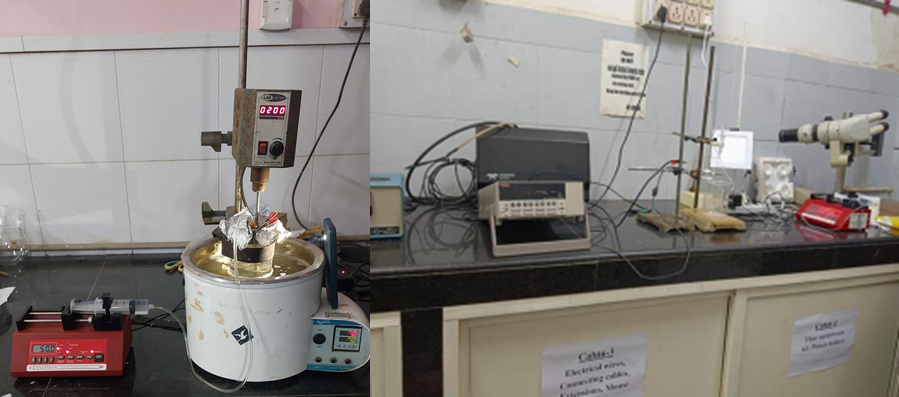
\includegraphics[width=0.8\linewidth]{udcafigs/Setups.png}
    \caption{Setup for Anti-Solvent and Electrospray systems}
    \label{fig:setups}
\end{figure}
\pagebreak
\newpage
\begin{figure}
    \centering
    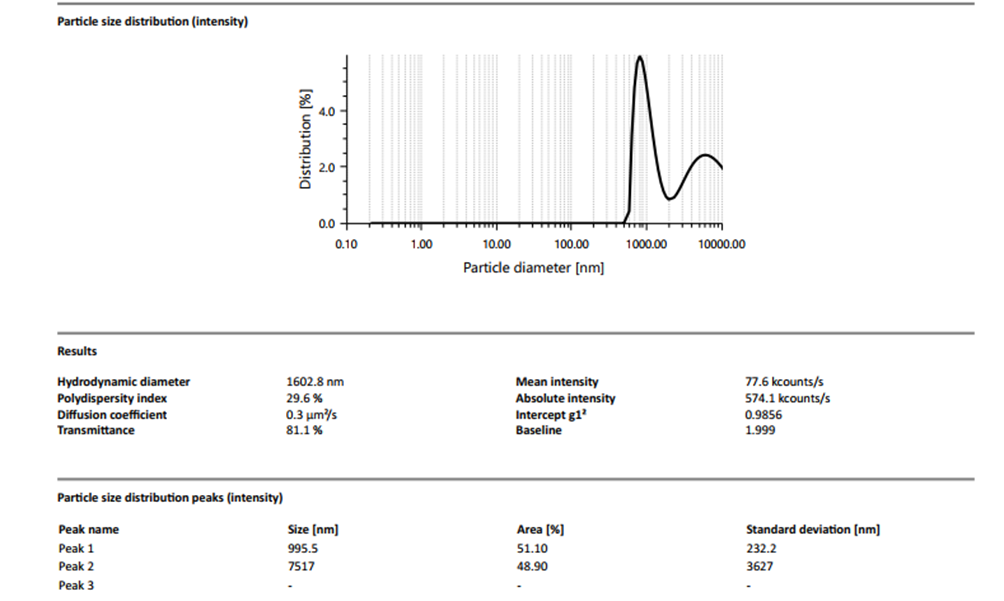
\includegraphics[width=0.8\linewidth]{udcafigs/Untreated-UDCA.png}
    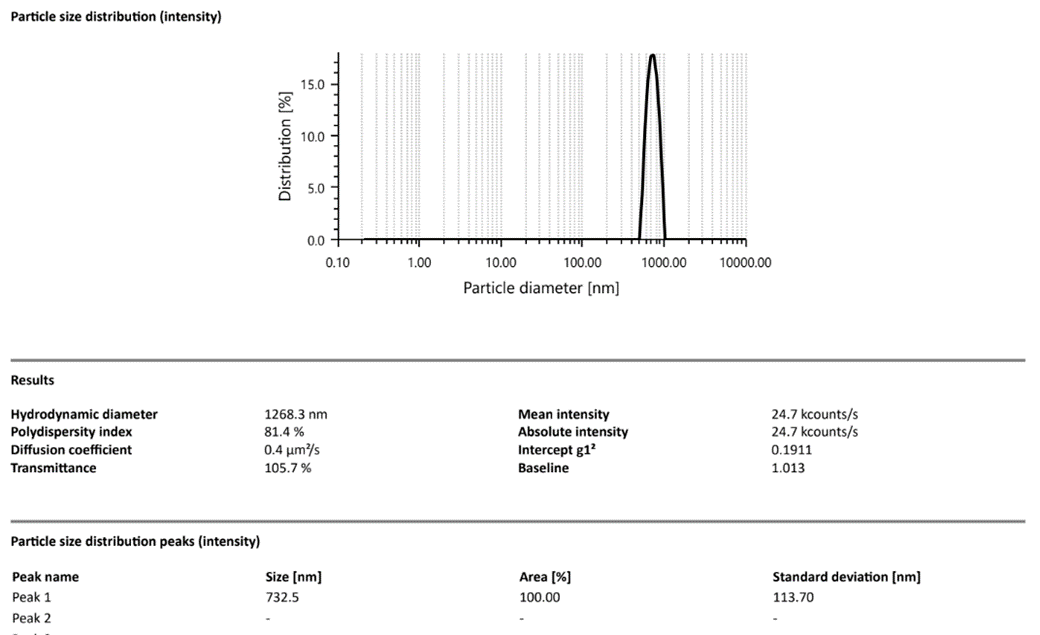
\includegraphics[width=0.8\linewidth]{udcafigs/Untreated-UDCA-Sample2.png}
    \caption{Untreated-UDCA: 2 Data Sets}
    \label{fig:untreated-UDCA}
\end{figure}
\pagebreak
\newpage
\begin{figure}
    \centering
    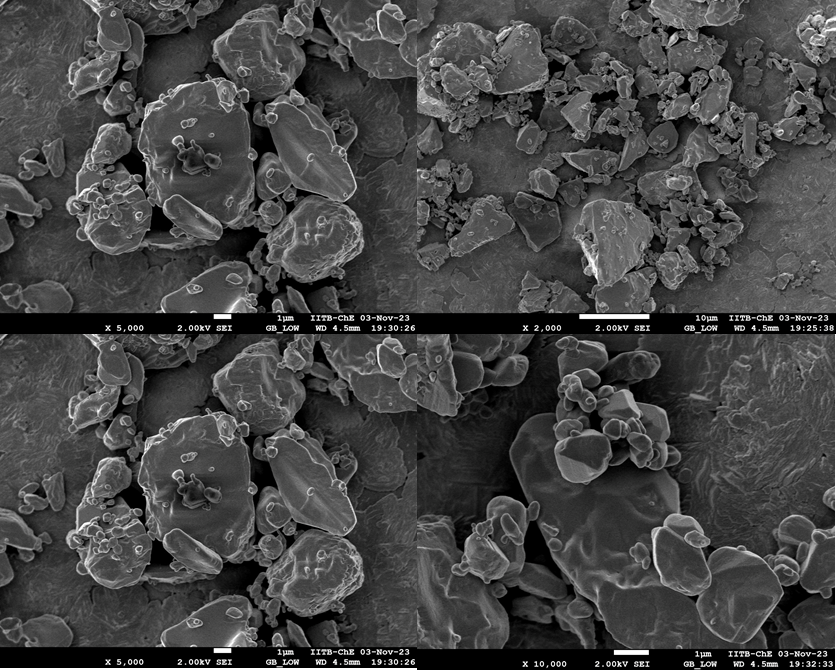
\includegraphics[width=0.8\linewidth]{udcafigs/SEM-Untreated-UDCA.png}
    \caption{Untreated-UDCA-SEM-Images}
    \label{fig:SEM-Untreated}
\end{figure}
\newpage
\begin{figure}
    \centering
    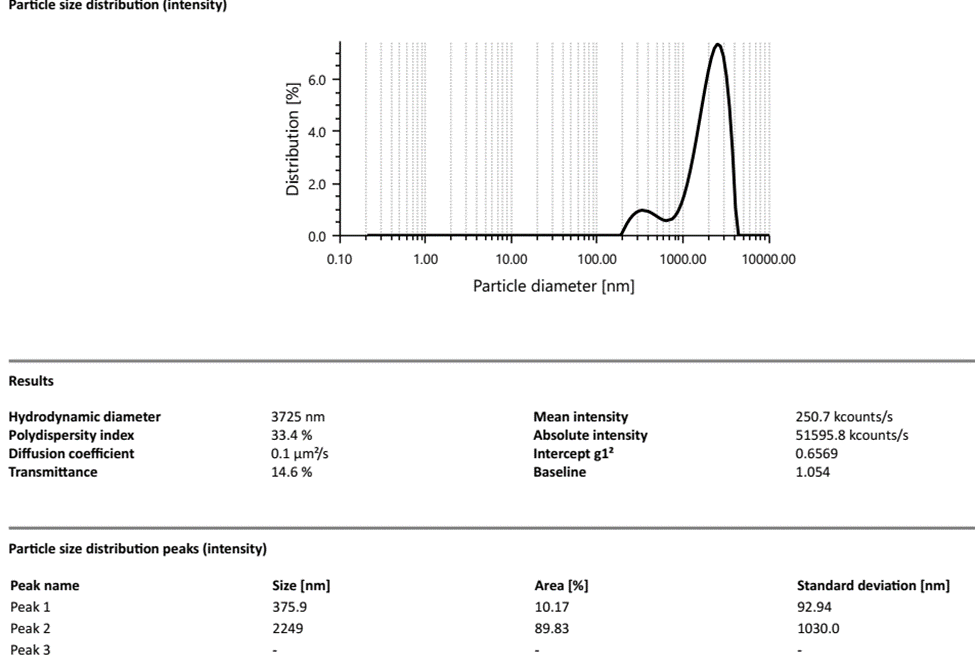
\includegraphics[width=0.8\linewidth]{udcafigs/Antisolve-UDCAw-o-HPMC.png}
    \caption{Antisolvent Method UDCA without HPMC}
    \label{fig:placeholder}
\end{figure}
\begin{figure}
    \centering
    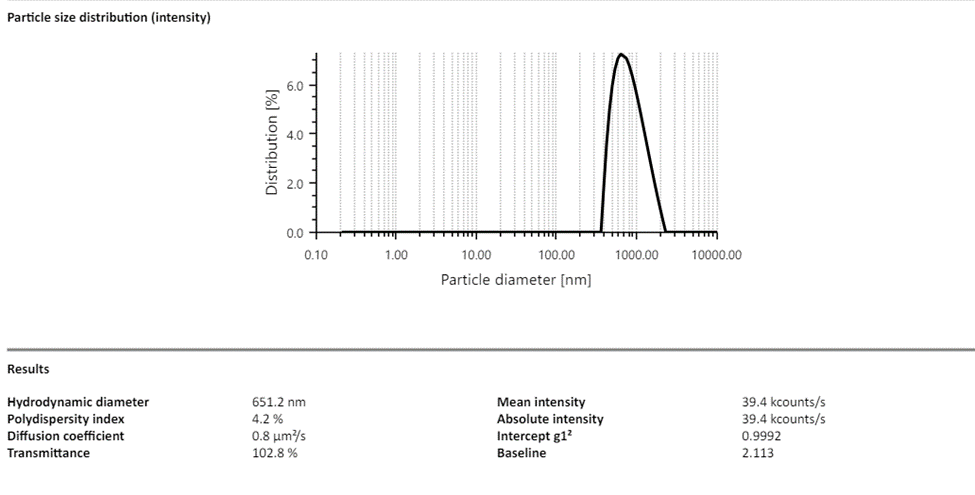
\includegraphics[width=0.8\linewidth]{udcafigs/DLS-HPMC-IPA.png}
    \caption{DLS of UDCA sample with HPMC and IPA}
    \label{fig:placeholder}
\end{figure}
\begin{figure}
    \centering
    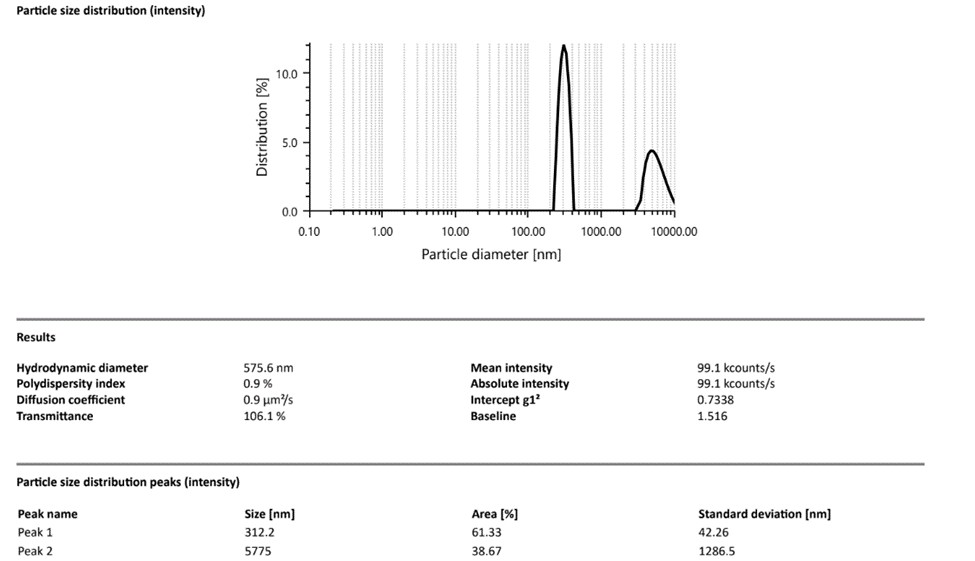
\includegraphics[width=0.8\linewidth]{udcafigs/Antisolvent-UDCA-With-HPMC-Ethanol.png}
    \caption{DLS of UDCA sample with HPMC and Ethanol}
    \label{fig:placeholder}
\end{figure}
\begin{figure}
    \centering
    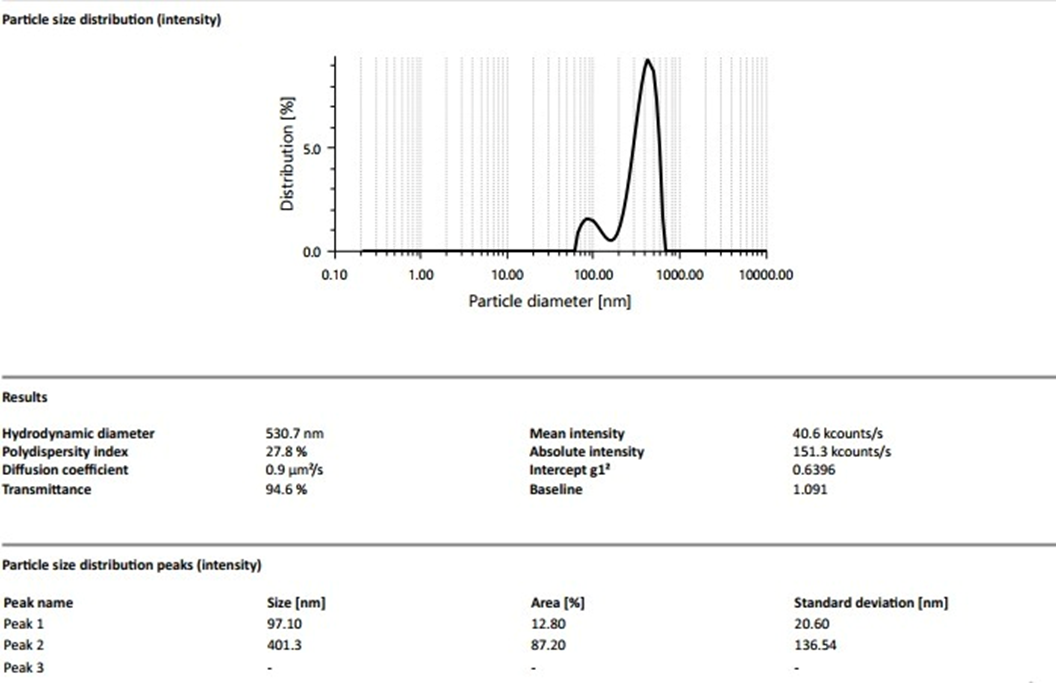
\includegraphics[width=0.8\linewidth]{udcafigs/With-Electrospray-HPMC.png}
    \caption{DLS of UDCA with HPMC and IPA generated using Electrospray}
    \label{fig:placeholder}
\end{figure}
\begin{figure}
    \centering
    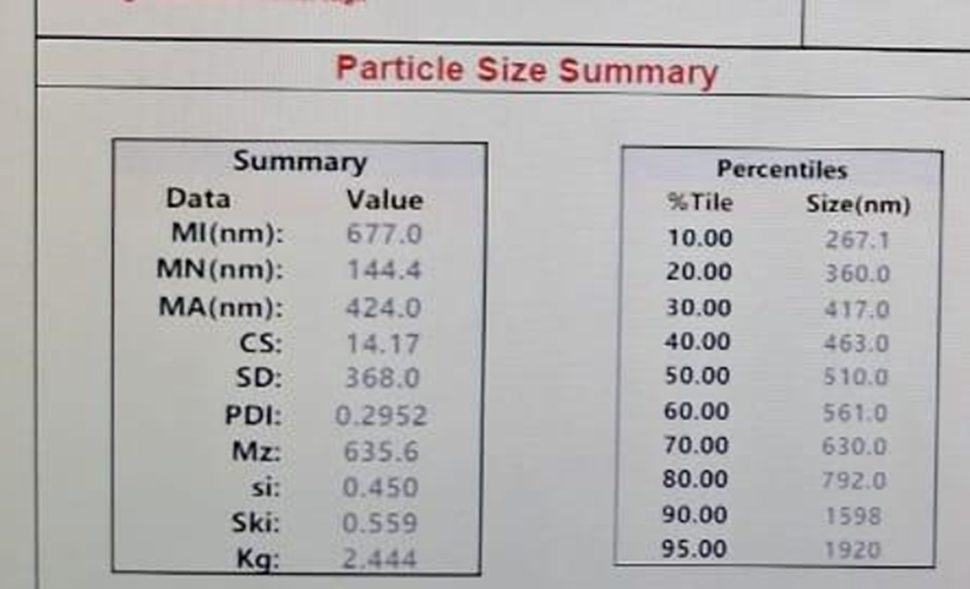
\includegraphics[width=0.45\linewidth]{udcafigs/HPH-HPMC.png}
        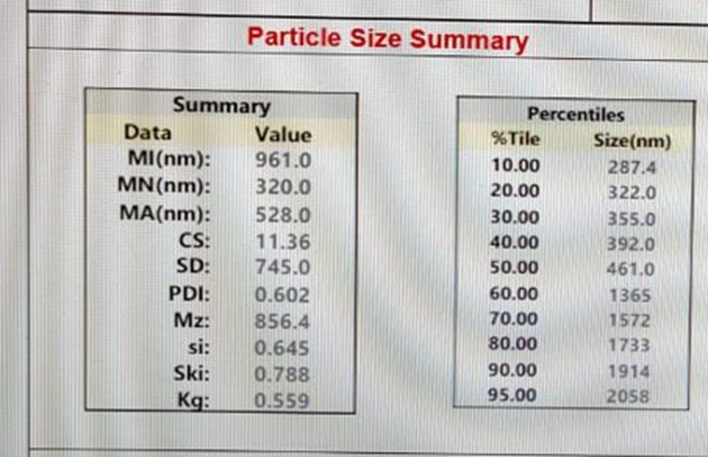
\includegraphics[width=0.45\linewidth]{udcafigs/HPH-withoutHPMC.png}
    \caption{HPH-HPMC and without HPMC results Results}
    \label{fig:HPH-HPMC}
\end{figure}



\end{document}
